\documentclass[12pt,]{article}
\usepackage[utf8]{inputenc}
\usepackage[T1]{fontenc}
\usepackage{mathptmx}
\usepackage{geometry}
\usepackage{mathtools}
\usepackage[english]{babel}
\usepackage{graphicx}
\usepackage{subcaption}
\usepackage{stackengine}
\usepackage[os=win]{menukeys}
\usepackage{hyperref}
\usepackage{minted}
\usepackage{xcolor}
\usepackage{tikz}
\usepackage[yyyymmdd,hhmmss]{datetime}
\usepackage{etoolbox}
\usepackage[inline]{enumitem}
\usepackage{pdfpages}

\newcommand{\WindowsLogo}{\raisebox{-0.1em}{
\includegraphics[height=0.8em]{images/logo/Windows_3_logo_simplified}}}
%\newcommand{\PowerLogo}{\raisebox{-0.1em}{\includegraphics[height=0.8em]{images/logo/power}}}
\newcommand{\WinKey}{\keys{\WindowsLogo}}
\newcommand{\PowerKey}{\keys{\PowerLogo}}

\patchcmd{\thebibliography}{\section*{\refname}}{}{}{}

\newcommand{\ShowOsVersion}{
	\immediate\write18{\unexpanded{foo=`uname -sro` && echo "${foo}" > tmp.tex}}
	\input{tmp}\immediate\write18{rm tmp.tex}
}

\newcommand{\ShowTexVersion}{
	\immediate\write18{\unexpanded{foo=`pdflatex -version | head -n1 | cut -d' ' -f1,2` && echo "${foo}" > tmp.tex}}
	\input{tmp}\immediate\write18{rm tmp.tex}
}

\addto\captionsenglish{\renewcommand{\contentsname}{Daftar Isi}}
\addto\captionsenglish{\renewcommand{\figurename}{Gambar}}

\hypersetup{
	colorlinks=true, %set true if you want colored links
	linktoc=all,     %set to all if you want both sections and subsections linked
	linkcolor=blue,  %choose some color if you want links to stand out
	urlcolor=blue,   %url color
}

\geometry{
	a4paper,
	left=10mm,
	right=10mm,
	top=10mm,
	bottom=15mm,
}

\title{\LARGE \bf
	Preview/Prototype Sistem Server IoT\\
}

\author{Achmadi ST MT}

\date{}

\hypersetup{citecolor=black}

\definecolor{LightGray}{gray}{0.95}

%\pagecolor[rgb]{0.1,0.1,0.1}
%\color[rgb]{1,1,1}

\begin{document}
	\thispagestyle{empty}
	
	\begin{titlepage}
		\centering
		\vfill
		\vfill
		\maketitle
		\vfill
		
\includegraphics[width=200pt]{images/logoviblab}
		\vfill
		\vfill
		Update: {\today} \currenttime \\
	\end{titlepage}
	
	%%%%%%%%%%%%%%%%%%%%%%%%%%%%%%%%%%%%%%%%%%%%%%%%%%%%%%%%%%%%%%%%%
	
	\section{Skema Pertama: Alur Data Via HTTP/HTTPS}
	
	Berikut skema prototype server IOT:
	
	\begin{figure}[!ht]
		\centering
		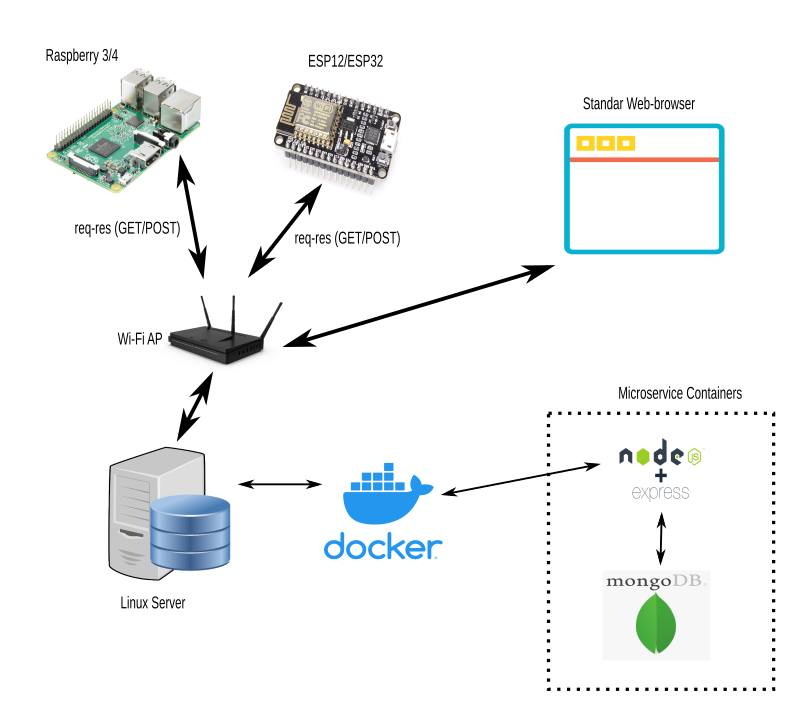
\includegraphics[width=500pt]{images/preview}
		\caption{Prototype Server}
	\end{figure}

	Spesifikasi untuk skema di atas:
	\begin{itemize}
		\item Raspberry Pi 3/4 dengan WiFi untuk agen IoT
		\item Board ESP8266/NodeMCU/ESP32 sebagai alternatif embedded agen IoT 
		\item Generic WiFi access point untuk penyedia WiFi
		\item Linux Server untuk wadah container.
		Untuk implementasi akhir akan dibangun dedicated server khusus.
		Alternatif lain akan menyewa penyedia layanan VPS.
		\item req-res adalah proses Request dan Respon via HTTP/GET atau HTTPS/POST
	\end{itemize}

	\newpage
	\section{Skema Kedua: Alur Data Via MQTT}
	
	Berikut skema prototype server IOT:
	
	\begin{figure}[!ht]
		\centering
		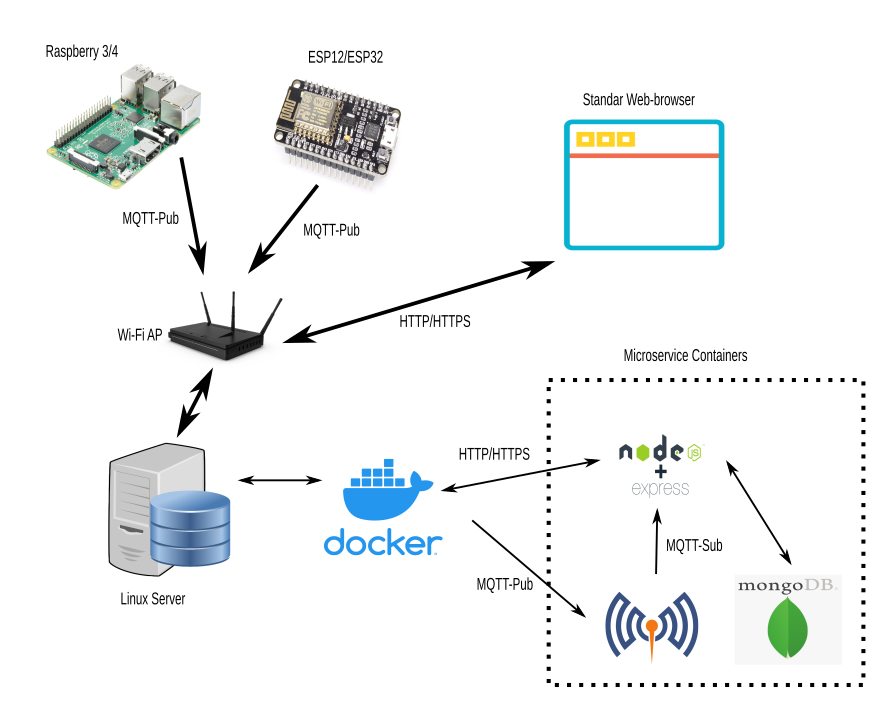
\includegraphics[width=500pt]{images/preview-mqtt}
		\caption{Prototype Server MQTT}
	\end{figure}
	
	Spesifikasi untuk skema di atas:
	\begin{itemize}
		\item Raspberry Pi 3/4 dengan WiFi untuk agen IoT
		\item Board ESP8266/NodeMCU/ESP32 sebagai alternatif embedded agen IoT 
		\item Generic WiFi access point untuk penyedia WiFi
		\item Linux Server untuk wadah container.
		Untuk implementasi akhir akan dibangun dedicated server khusus.
		Alternatif lain akan menyewa penyedia layanan VPS.
		\item MQTT-Pub adalah protocol pesan Publish semisal dari agen IoT ke Mosquitto (MQTT Broker)
		\item MQTT-Sub adalah protocol pesan Subscribe semisal dari MQTT Broker ke layanan web.
	\end{itemize}

	\newpage
	\section{Lampiran/Tambahan}
	
	Berikut beberapa informasi tambahan jika diperlukan:
	\begin{itemize}
		\item Sistem Operasi Prototype Server:
		\begin{itemize}
			\item Kernel: Linux 5.11.15-arch1-2 x86\_64 (Arch-Linux)
			\item SELinux: Belum dikonfigurasi
			\item iptables/nftables: Belum dikonfigurasi
		\end{itemize}
	
		\item Source tree prototype (jika perlu mereview):
		\begin{itemize}
			\item Docker prototype server:\\
			\url{https://github.com/VibrasticLab/ehealth-web/}
			
			\item ESP8266/NodeMCU agen IoT:\\
			\url{https://github.com/VibrasticLab/ehealth-iot/tree/master/esp8266-client/}
			
			\item Raspberry Pi 3/4 agen IoT: Menunggu tim pengembang hardware yang akan dipasang agen IoT:
		\end{itemize}
	
		\item API yang telah tersedia (sementara masih hanya diakses di jaringan lokal ITS):
		\begin{itemize}
			\item Home Page:\\
			\url{http://10.124.5.232/}
			
			\item Database management (hanya untuk masa pengembangan):\\
			\url{http://10.124.5.232:8081/}
			
			\item API GET untuk input data dari IoT device:\\
			\url{http://10.124.5.232/iotdata?devid=XXX&data=YYY}
			
			\item API POST untuk input data dari IoT device: Menyusul
			
			\item MQTT Publish untuk input data dari IoT device: Menyusul
		\end{itemize}
	
		\textbf{Catatan:} Prototype server belum dilengkapi UPS sehingga IP dapat berubah sewaktu-waktu
		jika listrik padam dan DHCP jurusan akan \textit{assign} IP saat kembali menyala.
	\end{itemize}
\end{document}
